\documentclass[11pt]{article}

\usepackage[a4paper,margin=2.5cm]{geometry}
\usepackage[utf8]{inputenc}
\usepackage[T1]{fontenc}
\usepackage{booktabs}
\usepackage{array}
\usepackage{longtable}
\usepackage{xcolor}
\usepackage{enumitem}
\usepackage{parskip}
\usepackage{graphicx}
\usepackage{caption}
% Multi-paragraph figure captions. Every figure also carries a SHORT optional caption
% (\caption[short]{long}): without it, a blank line inside \caption{} makes hyperref's
% nameref abort the build. Loading `caption` alone does not fix that.
\captionsetup{format=plain,justification=justified,font=small}
\graphicspath{{figs/}}
\usepackage{hyperref}
\hypersetup{
  colorlinks=true,
  linkcolor=blue!50!black,
  citecolor=blue!50!black,
  urlcolor=blue!50!black,
  pdftitle={Component S: Status, Capability and Remaining Work},
  pdfauthor={Component S Documentation}
}

\title{\textbf{Component S: A Statistical Emulator of Forest\\ Demography and Tree-Trait Diversity}\\
\large Status, capability, and remaining work}
\author{}
\date{}

\begin{document}

\maketitle

\begin{abstract}
\noindent
Component S is the slow, annual component of a hybrid land model for use inside an Earth System Model. Once per simulated year it replaces an explicit, individual-tree demography calculation with a trained statistical prediction: given a summary of how a patch of forest fared physically that year, it returns how many trees are alive and what functional traits the newly established ones carry. It is trained on the output of LPJmL-FIT, an individual- and trait-based dynamic global vegetation model, and validated out-of-sample against it.

\textbf{Current status.} Component S reproduces LPJmL-FIT's forest \emph{structure} globally at close to the achievable accuracy limit: tree density at $R^2 = 0.982$ per patch-year and $0.999$ per grid cell, and all four functional-trait distributions with pooled Kolmogorov--Smirnov distances below $0.012$. It runs on the complete seven tree plant-functional-type set, over both a historical and an SSP3-7.0 future-climate period, on 58{,}588 grid cells. Serialised artifacts are dependency-free and load in seconds.

\textbf{Principal open item.} Reproducing the \emph{level} of a quantity is not the same as reproducing its \emph{change} under warming, and Component S currently understates the warming-driven shift in wood density by about 37 percent. It is therefore a validated structural emulator and a not-yet-validated response emulator. Sections \ref{sec:standing} and \ref{sec:roadmap} state precisely what this permits today and what closing it requires.

This report is written for ecologists, geoscientists and vegetation modellers. Plain-language explanations of each statistical measure are given in Section \ref{sec:measures}; complete specifications of inputs, targets and model dimensions are tabulated in Sections \ref{sec:data} and \ref{sec:method} for readers who need to reproduce or couple to the component.
\end{abstract}

\tableofcontents
\newpage

\section{Purpose and design}

An Earth System Model needs the land surface to supply water, energy and carbon fluxes every timestep. Vegetation controls those fluxes, and vegetation itself changes on much longer timescales -- trees establish, compete, and die over decades to centuries. Resolving that demography explicitly, tree by tree, is what makes a model like LPJmL-FIT scientifically detailed and simultaneously far too slow to run repeatedly inside a coupled climate simulation at global scale.

The hybrid land model this work belongs to splits the problem by timescale:

\begin{itemize}[leftmargin=1.4em]
\item \textbf{F} -- a fast, differentiable, conserving daily biophysical core (photosynthesis, water and carbon fluxes), retained from LPJmL-FIT and reimplemented to be automatically differentiable.
\item \textbf{E} -- a surface-energy-balance and skin-temperature closure, which LPJmL-FIT lacks and a coupled model requires.
\item \textbf{S} -- \emph{this component}: the slow, annual demography and trait step, replaced by a trained statistical emulator.
\end{itemize}

Component S is called once per simulated year. It receives that year's physical summary from F and returns an updated forest: a tree count, and traits for new recruits. It answers two questions, and is built from two correspondingly different statistical models (Section \ref{sec:method}):

\begin{enumerate}[leftmargin=1.6em]
\item \textbf{How many trees are now alive in this patch?} A count, predicted by a distributional random forest.
\item \textbf{What traits do the new trees have?} A jointly consistent bundle of four functional traits per recruit, drawn from a conditional Gaussian copula.
\end{enumerate}

\textbf{Scope.} Component S covers \emph{trees}. Grasses in the same patch are handled by component F and are not discussed further. Traits are assigned to \emph{recruits}; mortality in the emulator is trait-blind, which is why the target for the trait model is LPJmL-FIT's \emph{survivor} trait distribution rather than its establishment distribution.

\section{Training data}
\label{sec:data}

\subsection{Source, coverage and scale}

The reference data is LPJmL-FIT output, not field observation: the objective is faithful emulation of a specific, well-characterised process model. Two independent realisations of each scenario exist, differing only in the stochastic seed, which makes the model's own irreducible randomness measurable (Section \ref{sec:floor}).

\begin{table}[h]
\centering
\caption{Reference data coverage and scale. ``Stems'' are individual tree-year records; ``patch-years'' are the rows the count model is trained on. Each grid cell contains 25 independently simulated patches, representing the natural spread of forest states within a cell.}
\label{tab:scale}
\small
\begin{tabular}{lccc}
\toprule
& Historical & Future climate & Pooled \\
\midrule
Scenario & observed climate & SSP3-7.0 & both \\
Period & 2000--2019 (20 yr) & 2020--2100 (81 yr) & --- \\
Grid & 0.5$^\circ$, 67{,}420 land cells & same & same \\
Patches per cell & 25 & 25 & 25 \\
Cells with usable tree data & 54{,}020 & 58{,}683 & 58{,}588 \\
Individual tree-year records (all) & 246{,}049{,}830 & 1{,}030{,}175{,}289 & $1.28 \times 10^{9}$ \\
\quad of which surviving stems & $1.98 \times 10^{8}$ & --- & --- \\
Patch-year rows (count target) & 22{,}467{,}348 & 99{,}028{,}310 & 121{,}495{,}658 \\
Independent seeds available & 2 & 2 & 2 \\
CO$_2$ treatment & transient & held at 409.63\,ppm from 2020 & --- \\
\bottomrule
\end{tabular}
\end{table}

The seven tree plant-functional types (PFTs) represented, all of which are included: tropical broadleaved evergreen; temperate needleleaved evergreen; temperate broadleaved evergreen; temperate broadleaved summergreen; boreal needleleaved evergreen; boreal broadleaved summergreen; boreal needleleaved summergreen (larch). Three grass types are present in the reference output but belong to component F.

\subsection{Recorded quantities: the per-tree, per-year record}
\label{sec:recorded}

LPJmL-FIT emits one row per living tree per year with the 29 fields below. This is the complete input universe from which everything else in this report is derived.

\begin{table}[h]
\centering
\caption{The 29 recorded fields per tree per year (LPJmL-FIT \texttt{ind} output). ``Role'' indicates how Component S uses the field: \emph{index} = identifies the record; \emph{driver} = aggregated into a model input; \emph{target} = predicted; \emph{diagnostic} = validated but not predicted in production; \emph{unused} = available but not currently consumed.}
\label{tab:recorded}
\small
\begin{tabular}{llll}
\toprule
Field & Meaning & Unit & Role \\
\midrule
\texttt{Cell} & grid cell index & --- & index \\
\texttt{Patch} & patch index within cell & --- & index \\
\texttt{Year} & simulation year & yr & index \\
\texttt{ID} & individual identifier & --- & index \\
\texttt{Type} & plant functional type (0--6 = trees) & --- & index / filter \\
\midrule
\texttt{npp} & net primary production & gC\,m$^{-2}$\,yr$^{-1}$ & driver \\
\texttt{gpp} & gross primary production & gC\,m$^{-2}$\,yr$^{-1}$ & driver \\
\texttt{transp} & transpiration & mm\,yr$^{-1}$ & unused \\
\texttt{wscal\_mean} & annual mean leaf-on water scalar (1 = unstressed) & --- & driver \\
\texttt{vegc} & total vegetation carbon & gC\,m$^{-2}$ & unused \\
\texttt{agb} & above-ground biomass & gC\,m$^{-2}$ & driver / diagnostic \\
\texttt{Height} & tree height & m & driver / diagnostic \\
\texttt{Age} & age at year end & yr & driver \\
\texttt{LAI} & within-crown leaf area index & m$^2$\,m$^{-2}$ & driver \\
\texttt{fpc\_ind} & foliar projective cover of the individual & --- & driver \\
\midrule
\texttt{SLA} & specific leaf area & m$^2$\,gC$^{-1}$ & \textbf{target} \\
\texttt{Wooddens} & wood density & gC\,m$^{-3}$ & \textbf{target} \\
\texttt{D95max} & sampled maximum 95\,\% rooting depth & cm & \textbf{target} \\
\texttt{minwscal} & drought-tolerance threshold & --- & \textbf{target} \\
\texttt{Longevity} & leaf longevity & yr & unused \\
\texttt{D95} & realised (depth-limited) 95\,\% rooting depth & cm & unused \\
\texttt{beta\_root} & root-profile shape parameter & --- & unused \\
\texttt{k\_root} & root-profile scaling & --- & unused \\
\midrule
\texttt{mort} & total mortality probability & --- & unused \\
\texttt{mort\_npp} & mortality from carbon starvation & --- & unused \\
\texttt{mort\_age} & mortality from age & --- & unused \\
\texttt{mort\_water} & mortality from water stress & --- & unused \\
\texttt{mort\_temp} & mortality from temperature stress & --- & unused \\
\texttt{isdead} & died this year (survivor filter) & 0/1 & filter \\
\bottomrule
\end{tabular}
\end{table}

Two practical notes for anyone re-deriving from this table. \texttt{agb} carries the individual density factor already applied, so a per-patch row sum is the stand total per unit area. The emitted \texttt{Age} is incremented at year end, so start-of-year age is $\texttt{Age}-1$; the mortality fields on the same row were evaluated at that earlier age.

\subsection{Model inputs: exactly what Component S is trained on}
\label{sec:inputs}

The two sub-models take different input sets. The count model sees the full patch state; the trait model deliberately sees only the environmental drivers and not the patch's own structure, because recruit traits are set by establishment conditions rather than by the existing stand.

\begin{table}[h]
\centering
\caption{Inputs to the \textbf{count} model (15 predictors), in the exact order the running model supplies them. ``Flux drivers'' come from component F for the year just simulated; ``patch state'' describes the stand at the start of the step; ``boundary'' is the slowly varying bioclimatic and soil context.}
\label{tab:count_inputs}
\small
\begin{tabular}{cllll}
\toprule
\# & Predictor & Meaning & Unit & Group \\
\midrule
1 & \texttt{bm\_inc\_cell} & annual carbon increment available to the stand & gC\,m$^{-2}$ & flux driver \\
2 & \texttt{growth\_eff} & growth efficiency (increment per unit leaf area) & gC\,m$^{-2}$ & flux driver \\
3 & \texttt{water\_stress} & $1 -$ mean leaf-on water scalar & --- & flux driver \\
4 & \texttt{soilmoist} & root-zone soil moisture, capacity-weighted & --- & flux driver \\
\midrule
5 & \texttt{hmean} & cover-weighted mean tree height & m & patch state \\
6 & \texttt{hmax} & maximum tree height & m & patch state \\
7 & \texttt{agb} & stand above-ground biomass & gC\,m$^{-2}$ & patch state \\
8 & \texttt{lai} & stand leaf area index & m$^2$\,m$^{-2}$ & patch state \\
9 & \texttt{fpc} & stand foliar projective cover & --- & patch state \\
10 & \texttt{age\_mean} & density-weighted mean cohort age & yr & patch state \\
11 & \texttt{n\_prev} & tree count at the start of the year & --- & patch state \\
\midrule
12 & \texttt{eco\_diag\_gdd\_5} & growing-degree days above 5\,$^\circ$C & $^\circ$C\,d & boundary \\
13 & \texttt{tas\_cold\_month} & mean temperature of the coldest month & $^\circ$C & boundary \\
14 & \texttt{soil\_depth} & plant-available soil depth & m & boundary \\
15 & \texttt{co2} & atmospheric CO$_2$ & ppm & boundary \\
\bottomrule
\end{tabular}
\end{table}

\begin{table}[h]
\centering
\caption{Inputs to the \textbf{trait} model (8 predictors in the deployed configuration). These are predictors 1--4 and 12--15 of Table \ref{tab:count_inputs}: the environmental drivers and the bioclimatic boundary, with the six patch-state descriptors and \texttt{n\_prev} deliberately excluded. An evaluated 14-predictor variant adds the six moisture descriptors listed beneath; its status is discussed in Section \ref{sec:roadmap}.}
\label{tab:trait_inputs}
\small
\resizebox{\textwidth}{!}{%
\begin{tabular}{cll}
\toprule
\# & Predictor & Group \\
\midrule
1--4 & \texttt{bm\_inc\_cell}, \texttt{growth\_eff}, \texttt{water\_stress}, \texttt{soilmoist} & flux drivers \\
5--8 & \texttt{eco\_diag\_gdd\_5}, \texttt{tas\_cold\_month}, \texttt{soil\_depth}, \texttt{co2} & boundary \\
\midrule
\multicolumn{3}{l}{\emph{Evaluated 14-predictor variant adds:}} \\
9--14 & \texttt{prec\_mean} (mean precipitation), \texttt{eco\_diag\_p\_pet\_ratio} (precipitation / potential & moisture \\
 & evapotranspiration), \texttt{eco\_diag\_pet\_mean} (potential evapotranspiration), & descriptors \\
 & \texttt{eco\_diag\_vpd\_mean} (vapour-pressure deficit), \texttt{pr\_cv\_monthly} (monthly & \\
 & precipitation variability), \texttt{humid\_mean} (specific humidity) & \\
\bottomrule
\end{tabular}%
}
\end{table}

\subsection{Prediction targets}

\begin{itemize}[leftmargin=1.4em]
\item \textbf{Count model:} \texttt{n\_living}, the number of living trees in a patch at year end (observed range 1--48).
\item \textbf{Trait model, production:} the joint distribution of \texttt{SLA}, \texttt{Wooddens}, \texttt{D95max}, \texttt{minwscal} over recruits. These four are exactly the traits LPJmL-FIT samples at establishment, and they map onto the carbon pools the coupled model requires.
\item \textbf{Trait model, diagnostic:} \texttt{agb} and \texttt{Height} per stem, validated identically but \emph{never} written into the production artifact, so an error in them cannot propagate into a coupled run.
\end{itemize}

\section{Method and model dimensions}
\label{sec:method}

\subsection{Counts: a distributional random forest}

A single decision tree splits the input space by asking successive threshold questions (``is growth efficiency above this value?''), ending in a leaf holding the training rows that satisfied all of them. A random forest grows many such trees, each on a different random subsample of rows and considering a random subset of predictors at each split, and combines them. The randomisation is what prevents the ensemble from memorising individual rows.

\emph{Distributional} means each leaf retains the full set of training values that reached it, not only their mean. A prediction is therefore a weighted empirical distribution over outcomes, from which a mean, a quantile, or a random draw can be taken. This matters here because forest demography is genuinely stochastic: the useful answer is ``how many trees are plausible in this situation,'' not only the single most likely number.

\subsection{Traits: a conditional Gaussian copula}

The four traits are correlated -- dense wood tends to accompany particular leaf economics -- so drawing them independently would generate combinations that never occur in nature or in LPJmL-FIT. A copula separates the problem into the \emph{shape} of each trait's own distribution and the \emph{dependence} between traits:

\begin{enumerate}[leftmargin=1.6em]
\item Draw four correlated standard normal values, $z \sim N(0, I)$, and correlate them as $z_c = L z$, where $L$ is the Cholesky factor of the trait correlation matrix $R = L L^{\mathsf{T}}$.
\item Convert each to a uniform number on $[0,1]$ via the normal cumulative distribution function, $u = \Phi(z_c)$. These four uniforms carry the dependence but no marginal shape.
\item Map each uniform through the corresponding trait's own conditional distribution -- supplied by a per-trait distributional random forest conditioned on the 8 environmental predictors of Table \ref{tab:trait_inputs} -- to obtain the trait value.
\end{enumerate}

The result is a recruit whose four traits are individually correctly distributed for its environment \emph{and} jointly consistent with one another.

\subsection{Dimensions of the deployed models}

\begin{table}[h]
\centering
\caption{Deployed model dimensions. \texttt{mtry} is the number of predictors considered at each split, set automatically to $\mathrm{round}(\sqrt{p})$. Minimum leaf size and maximum depth together limit how finely the forest may partition the input space, which is the main guard against memorising individual training rows. Artifacts are plain-text, dependency-free, and load without any external library.}
\label{tab:dims}
\small
\resizebox{\textwidth}{!}{%
\begin{tabular}{lcc}
\toprule
& Count model & Trait model (per axis) \\
\midrule
Model type & distributional random forest & DRF marginals + Gaussian copula \\
Predictors ($p$) & 15 & 8 \\
Targets & 1 (\texttt{n\_living}) & 4 production ($+$ 2 diagnostic) \\
Trees per forest & 150 & 60 \\
Maximum depth & 16 & 14 \\
Minimum leaf size & 20 & 20 \\
Rows subsampled per tree & 200{,}000 & 50{,}000 \\
\texttt{mtry} (predictors tried per split) & 4 & 3 \\
Copula dependence & --- & $4 \times 4$ correlation matrix, Cholesky factored \\
Serialised size & 51.6\,MB & 129\,MB \\
Training rows & $1.21 \times 10^{8}$ patch-years (pooled) & $1.98 \times 10^{8}$ surviving stems (hist.) \\
\bottomrule
\end{tabular}%
}
\end{table}

\section{Validation design}
\label{sec:validation}

Four independent checks are applied. Each answers a different question, and they are reported separately rather than merged into one score.

\paragraph{1. Held out by location.} Every grid cell is assigned to one of five groups. Each group is set aside in turn, a fresh model is trained on the remaining cells only, and that model predicts the withheld group. Every cell in the data set is therefore predicted exactly once by a model that never saw it. This is the basis for all headline numbers in Section \ref{sec:results}.

\paragraph{2. Held out by contiguous region (blocked).} Groups assigned by cell index are spatially scattered, so a withheld cell usually has trained neighbours 50\,km away in essentially the same climate -- and part of the apparent skill is then spatial interpolation rather than learned environmental response. The blocked design withholds entire $15^\circ \times 5^\circ$ blocks so that a cell's neighbours are withheld with it. Comparing the two designs separates real response from interpolation, and the result is reported in Section \ref{sec:standing}.

\paragraph{3. Held out by climate period.} The model is trained on the historical period alone and evaluated on the future-climate period it has never seen, and vice versa. This tests transfer to a different climate regime rather than to a different place.

\paragraph{4. Against the reference model's own repeatability -- the noise floor.}
\label{sec:floor}
LPJmL-FIT is stochastic: rerunning identical climate at an identical location with a different random seed yields a different, equally valid forest. No predictor that sees climate rather than the random-number stream can match either run exactly. That limit is measurable as the agreement between two seeds, and it is the correct standard against which to judge the emulator -- an emulator at the noise floor cannot be improved on, whatever its raw score.

The comparison is made attenuation-aware. Two reliabilities are estimated: the emulator's self-consistency (splitting its predictions at each location into interleaved halves and correlating the half-medians, then applying the standard correction for having used half the data) and the reference model's seed-to-seed reliability. The attainable \textbf{ceiling} is the geometric mean of the two, $\sqrt{\rho_P \rho_Y}$ -- looking through two imperfect windows is blurrier than either alone but not the sum of both blurs. The emulator's score divided by that ceiling is reported as $r_\mathrm{center}$; a value near 1 means the remaining error is irreducible rather than a modelling deficiency.

\section{Statistical measures used in this report}
\label{sec:measures}

\begin{description}[leftmargin=0em,style=nextline,itemsep=0.35em]
\item[$R^2$ (coefficient of determination)] The fraction of the variation in the true values that the prediction accounts for. $1.0$ is perfect; $0$ is no better than always predicting the overall mean. $R^2 = 0.98$ means 98\,\% of the variation is captured.
\item[RMSE (root-mean-square error)] The typical size of an individual miss, in the same units as the quantity itself, with large misses weighted more heavily than small ones. An RMSE of $0.69$ trees means a typical patch-level count error below one tree.
\item[Correlation ($r$, Pearson; $\rho$, Spearman)] How well predicted and true values move together. Pearson uses the values; Spearman uses only their rank order and so is insensitive to a monotonic distortion of scale. Reporting both distinguishes ``wrong ordering'' from ``right ordering, wrong scale''.
\item[Kolmogorov--Smirnov distance (KS)] The largest gap between two cumulative distributions -- a whole-shape comparison rather than a comparison of averages. $0$ is identical; $1$ is disjoint. Values below $\sim$0.02 indicate distributions that are difficult to distinguish. KS computed at a single grid cell is inherently larger than KS pooled globally, because one cell holds far fewer trees; the two must not be compared with each other.
\item[nqrmse] RMSE divided by the quantity's own interquartile range, so that traits in different units become comparable. It is unsuitable for strongly heavy-tailed quantities such as biomass, where KS should be read instead.
\item[Prediction-spread ratio] The standard deviation of the predictions divided by that of the truth. $1.0$ means the model reproduces the real geographic spread of a trait; below $1.0$ means it hedges toward the middle and under-represents genuine extremes.
\item[$r_\mathrm{center}$] Skill relative to the attainable ceiling of Section \ref{sec:floor}, rather than to a hypothetical perfect prediction.
\end{description}

\section{Results}
\label{sec:results}

All numbers below are held out by location (design 1), on the complete seven-PFT tree set. Cell counts differ slightly between tables because each reports the subset with sufficient data for that particular computation.

\subsection{Tree density}

\begin{table}[h]
\centering
\caption{Tree-count accuracy. ``Per patch-year'' pools every patch and year into one calculation -- the hardest framing. ``Per grid cell'' scores each cell's own year-to-year trajectory separately and then averages, which rewards tracking local dynamics.}
\label{tab:counts}
\small
\begin{tabular}{lccc}
\toprule
& Historical & Future climate & Pooled \\
\midrule
Patch-year rows / cells & 22.5\,M / 53{,}699 & 99.0\,M / 58{,}496 & 121.5\,M / 58{,}588 \\
$R^2$, held out by location, per patch-year & \textbf{0.9826} & \textbf{0.9823} & \textbf{0.9824} \\
RMSE (trees) & 0.689 & 0.698 & 0.697 \\
$R^2$, held out by climate period & 0.982 & 0.9818 & --- \\
$R^2$, per grid cell & 0.9988 & 0.9989 & 0.9989 \\
Mean bias (trees) & $+0.003$ & $+0.001$ & $+0.000$ \\
\bottomrule
\end{tabular}
\end{table}

Held-out accuracy equals in-sample accuracy to four decimal places, so the count model is not memorising locations. Held-out-by-period accuracy is indistinguishable from held-out-by-location accuracy, so it transfers to a climate regime it was not trained on. A seed-to-seed noise floor for counts is available ($\approx 0.99$) but is computed on cell totals pooled over patches and years, whereas the model is scored per patch-year; it is too generous a comparison to quote as this model's ceiling, and a matched per-patch-year floor is outstanding.

\begin{figure}[ht]
\centering
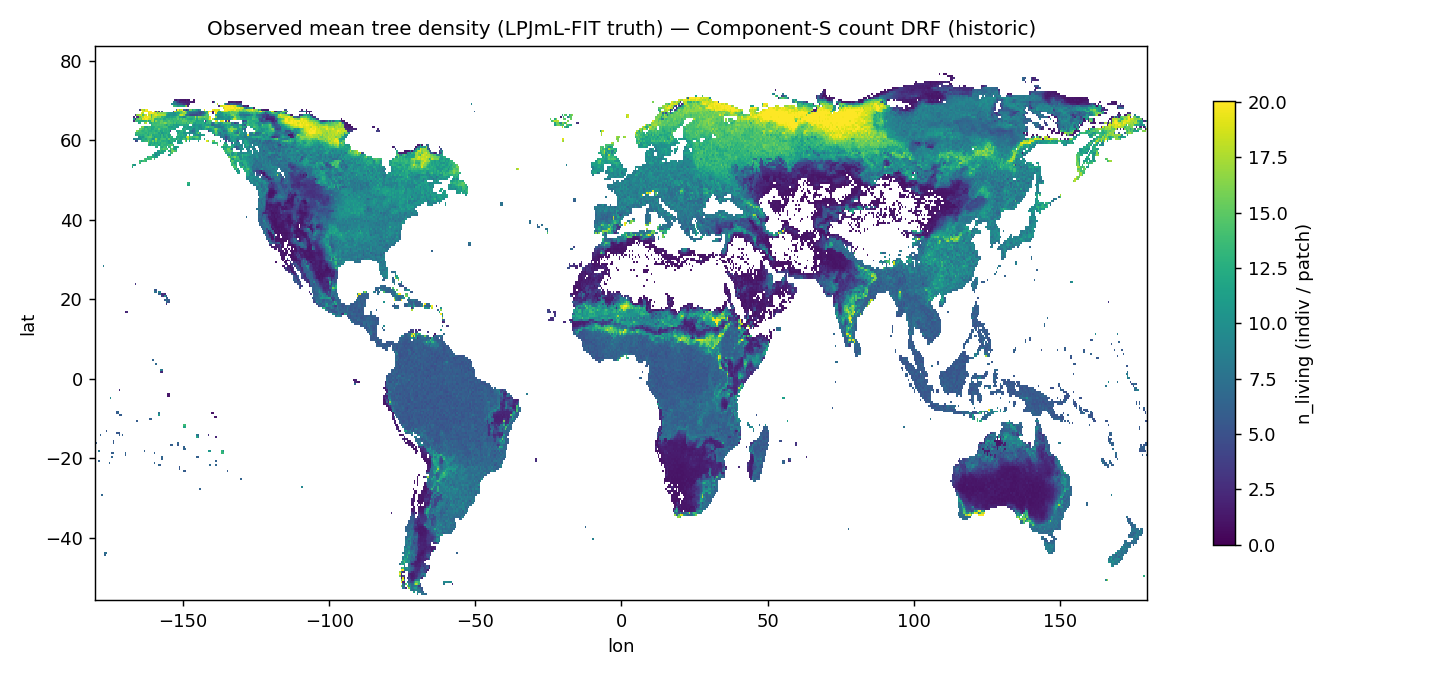
\includegraphics[width=0.92\textwidth]{count_map_observed.png}
\caption[Reference map: mean living trees per patch]{\textbf{What is shown.} The reference field to be reproduced: mean number of living trees per patch, per grid cell, from LPJmL-FIT over the historical period. Horizontal axis is longitude, vertical axis latitude; each pixel is one 0.5$^\circ$ cell. Bright yellow = many trees, dark purple = few, white = no living trees recorded (desert, ice).

\textbf{What it tells us.} This is the target, shown so the next two figures can be read against it. Its pattern is also a sanity check on the reference data: dense tropical, boreal and temperate forest belts, empty Sahara, Arabian Peninsula, central Australia and ice sheets.}
\label{fig:count_observed}
\end{figure}

\begin{figure}[ht]
\centering
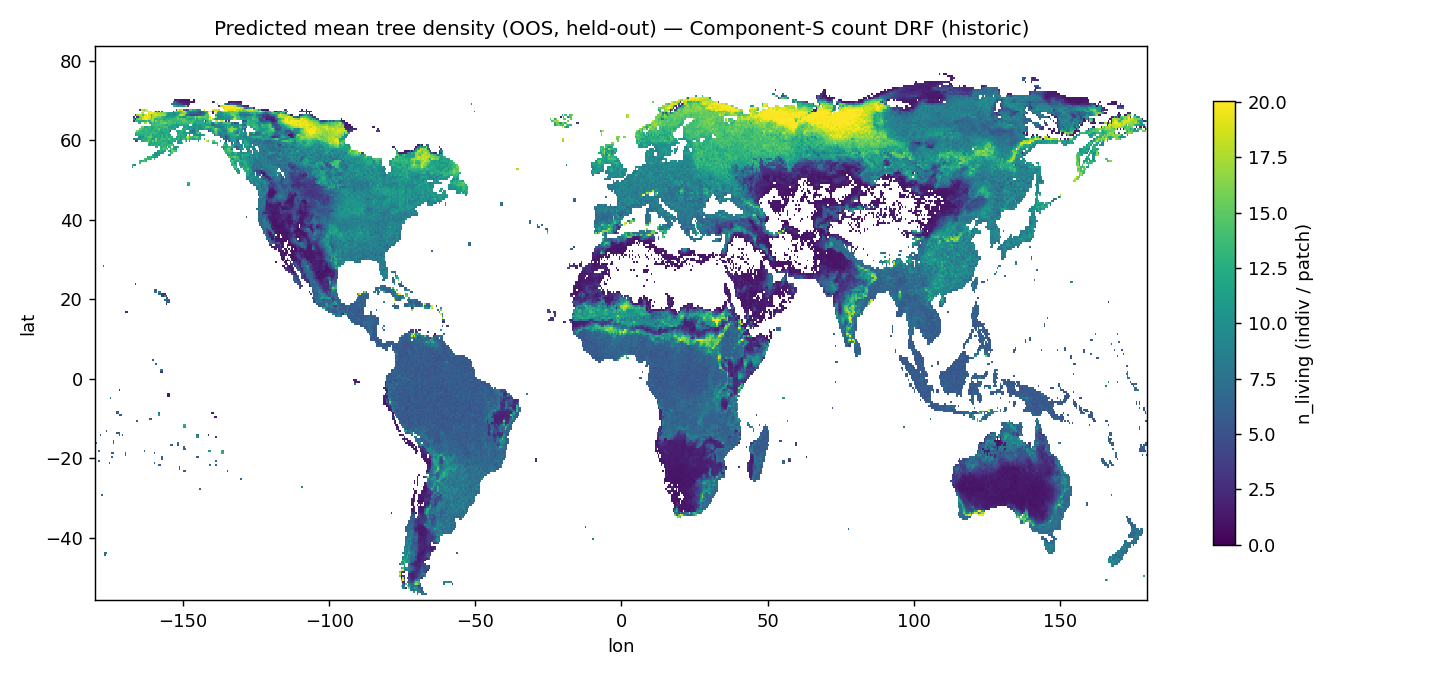
\includegraphics[width=0.92\textwidth]{count_map_predicted.png}
\caption[Predicted tree density, same scale]{\textbf{What is shown.} Component S's prediction of the same quantity, on the same colour scale and axes as Figure \ref{fig:count_observed}. Every pixel was withheld from the training data of the model that predicted it, so this is genuinely out-of-sample.

\textbf{What it tells us.} The two maps are close to indistinguishable at this scale -- forest belts and desert margins fall in the right places at the right intensities. This is the $R^2 = 0.9826$ of Table \ref{tab:counts} made visible. The eye judges gross pattern well and small systematic offsets poorly, which is why Figure \ref{fig:count_bias} follows.}
\label{fig:count_predicted}
\end{figure}

\begin{figure}[ht]
\centering
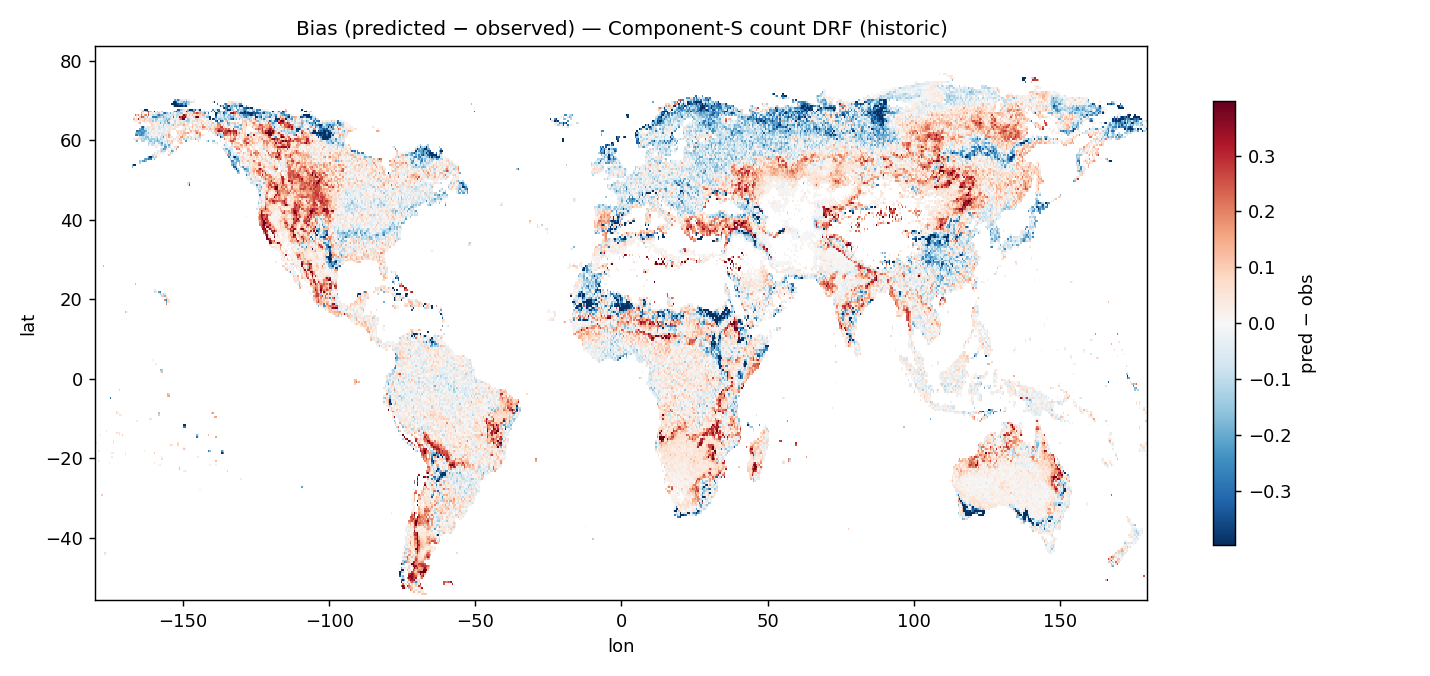
\includegraphics[width=0.92\textwidth]{count_map_bias.png}
\caption[Prediction error map]{\textbf{What is shown.} Predicted minus observed tree density at every location, on a diverging scale centred at zero: white = no detectable error, the two colour directions = over- and under-prediction, saturation = error magnitude. ``Bias'' here is the signed difference, as distinct from RMSE, which measures typical error size irrespective of sign.

\textbf{What it tells us.} Most of the land surface is white, so the high pooled $R^2$ reflects broadly distributed accuracy rather than large errors cancelling between regions. Residual error concentrates along the \emph{boreal tree line}, the sharp transition from closed forest to tundra -- the expected location, since a small error in predicted environment there produces a large error in tree number. The model's weakness sits at a physically meaningful ecological boundary rather than being scattered unexplainably.}
\label{fig:count_bias}
\end{figure}

\begin{figure}[ht]
\centering
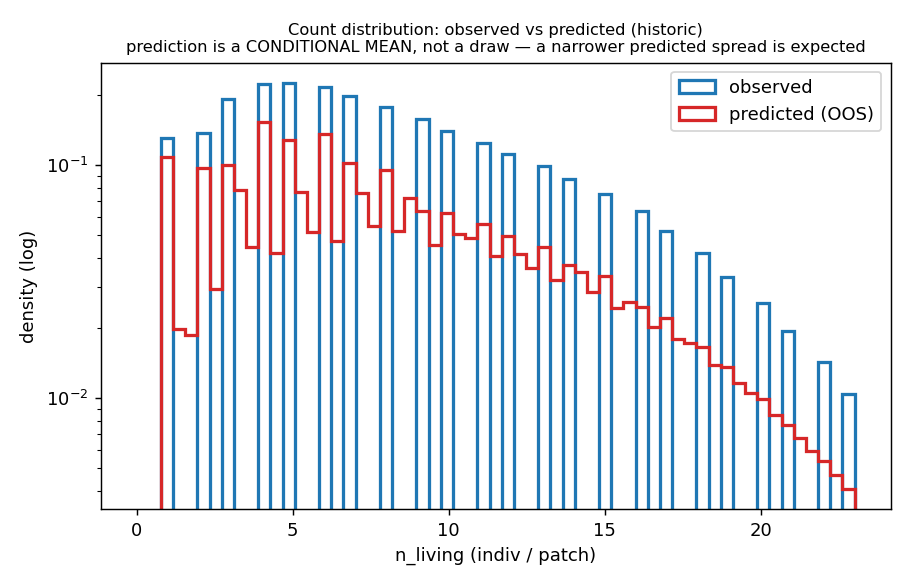
\includegraphics[width=0.75\textwidth]{count_distribution.png}
\caption[Distribution of tree counts per patch]{\textbf{What is shown.} The frequency of each possible tree count per patch, true versus predicted, pooled over all withheld patch-years. Horizontal axis is the count; vertical axis is how many patch-years had it, on a \emph{logarithmic} scale (each equal step upwards is a tenfold increase), so that both common low counts and rare high counts remain visible.

\textbf{What it tells us.} The curves overlap closely, so the model reproduces the whole spread of outcomes -- including how often unusually sparse or crowded patches occur -- and not only the mean. Where they part, the predicted curve is slightly \emph{narrower}. That is expected: the emulator returns the central tendency for each situation, while the reference model also adds genuine patch-to-patch stochasticity on top. The same effect is quantified for traits by the prediction-spread ratio.}
\label{fig:count_distribution}
\end{figure}

\begin{figure}[ht]
\centering
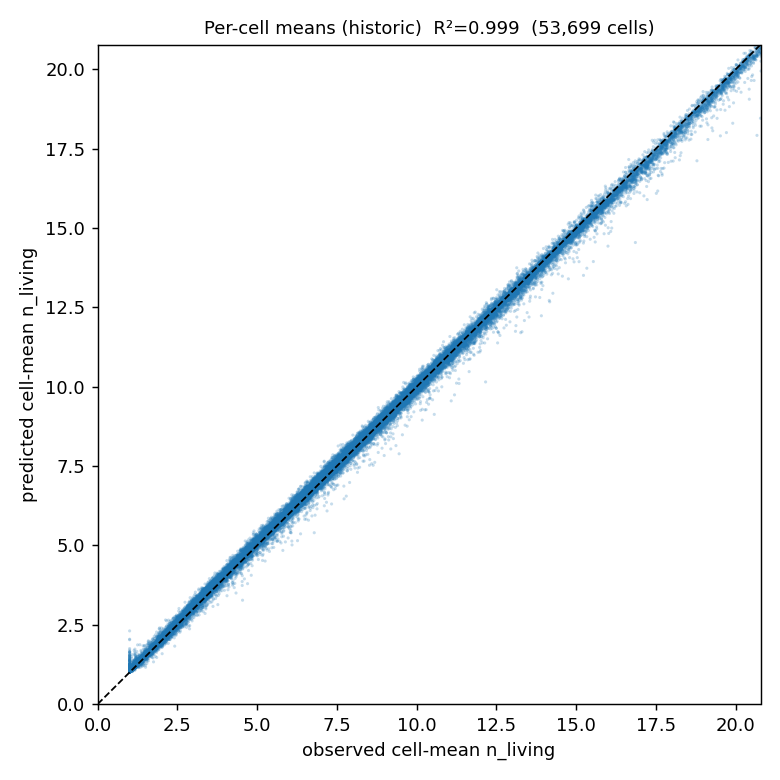
\includegraphics[width=0.62\textwidth]{count_percell_scatter.png}
\caption[Per-cell predicted versus true mean tree count]{\textbf{What is shown.} Each of 53{,}699 dots is one grid cell (not one tree, not one patch). Horizontal position is that cell's true mean tree count over its 25 patches and all years; vertical position is the held-out prediction. The dashed diagonal is perfect agreement; above it means over-prediction, below means under-prediction.

\textbf{What it tells us.} Dots lie on the diagonal across the full range from sparse to dense forest, with no curvature (which would indicate the model compressing extremes toward the middle) and no fanning (which would indicate accuracy varying with forest type). This is the per-cell $R^2 = 0.9988$ of Table \ref{tab:counts}. Note that averaging over years makes this a test of \emph{spatial} accuracy; it says nothing about accuracy of change over time, which is weaker (Section \ref{sec:standing}).}
\label{fig:count_percell}
\end{figure}

\clearpage
\subsection{Functional traits}

\begin{table}[h]
\centering
\caption{Per-trait accuracy against the attainable ceiling, historical period, 52{,}165 cells. ``Noise floor'' is seed-to-seed reliability alone; ``Ceiling'' additionally accounts for the emulator's own self-consistency and is therefore slightly higher; ``Gap'' is Ceiling minus Raw.}
\label{tab:traits}
\small
\begin{tabular}{lcccccc}
\toprule
Trait & Raw $r$ & Noise floor & Ceiling & Gap & $r_\mathrm{center}$ & Spread ratio \\
\midrule
Specific leaf area (\texttt{SLA}) & 0.881 & 0.973 & 0.986 & 0.104 & \textbf{0.894} & 0.907 \\
Wood density (\texttt{Wooddens}) & 0.814 & 0.937 & 0.964 & 0.150 & \textbf{0.844} & 0.678 \\
Rooting depth (\texttt{D95max}) & 0.791 & 0.833 & 0.909 & 0.118 & \textbf{0.870} & 0.714 \\
Drought tolerance (\texttt{minwscal}) & 0.945 & 0.973 & 0.986 & 0.041 & \textbf{0.958} & 0.970 \\
\bottomrule
\end{tabular}
\end{table}

\begin{table}[h]
\centering
\caption{Whole-distribution trait fidelity across scenarios: pooled Kolmogorov--Smirnov distance (global shape), median per-cell KS (local shape), and per-cell correlation. Diagnostic axes are marked.}
\label{tab:traits2}
\small
\begin{tabular}{lcccccc}
\toprule
& \multicolumn{2}{c}{Pooled KS} & \multicolumn{2}{c}{Median per-cell KS} & \multicolumn{2}{c}{Per-cell $r$} \\
\cmidrule(lr){2-3}\cmidrule(lr){4-5}\cmidrule(lr){6-7}
Axis & Hist. & Future & Hist. & Future & Hist. & Future \\
\midrule
\texttt{SLA} & 0.0051 & 0.0052 & 0.168 & 0.168 & 0.880 & 0.903 \\
\texttt{Wooddens} & 0.0052 & 0.0048 & 0.127 & 0.135 & 0.812 & 0.814 \\
\texttt{D95max} & 0.0069 & 0.0018 & 0.163 & 0.158 & 0.789 & 0.770 \\
\texttt{minwscal} & 0.0115 & 0.0040 & 0.146 & 0.150 & 0.944 & 0.962 \\
\texttt{agb} [diag] & 0.0116 & 0.0090 & 0.088 & 0.098 & 0.864 & 0.869 \\
\texttt{Height} [diag] & 0.0086 & 0.0059 & 0.062 & 0.077 & 0.954 & 0.954 \\
\bottomrule
\end{tabular}
\end{table}

Drought tolerance and specific leaf area are close to their ceilings. Wood density has the largest gap and the lowest spread ratio, meaning it under-represents genuine geographic variation; rooting depth is similar but milder. Every axis matches in global distributional shape (pooled KS $\le 0.012$).

\begin{figure}[ht]
\centering
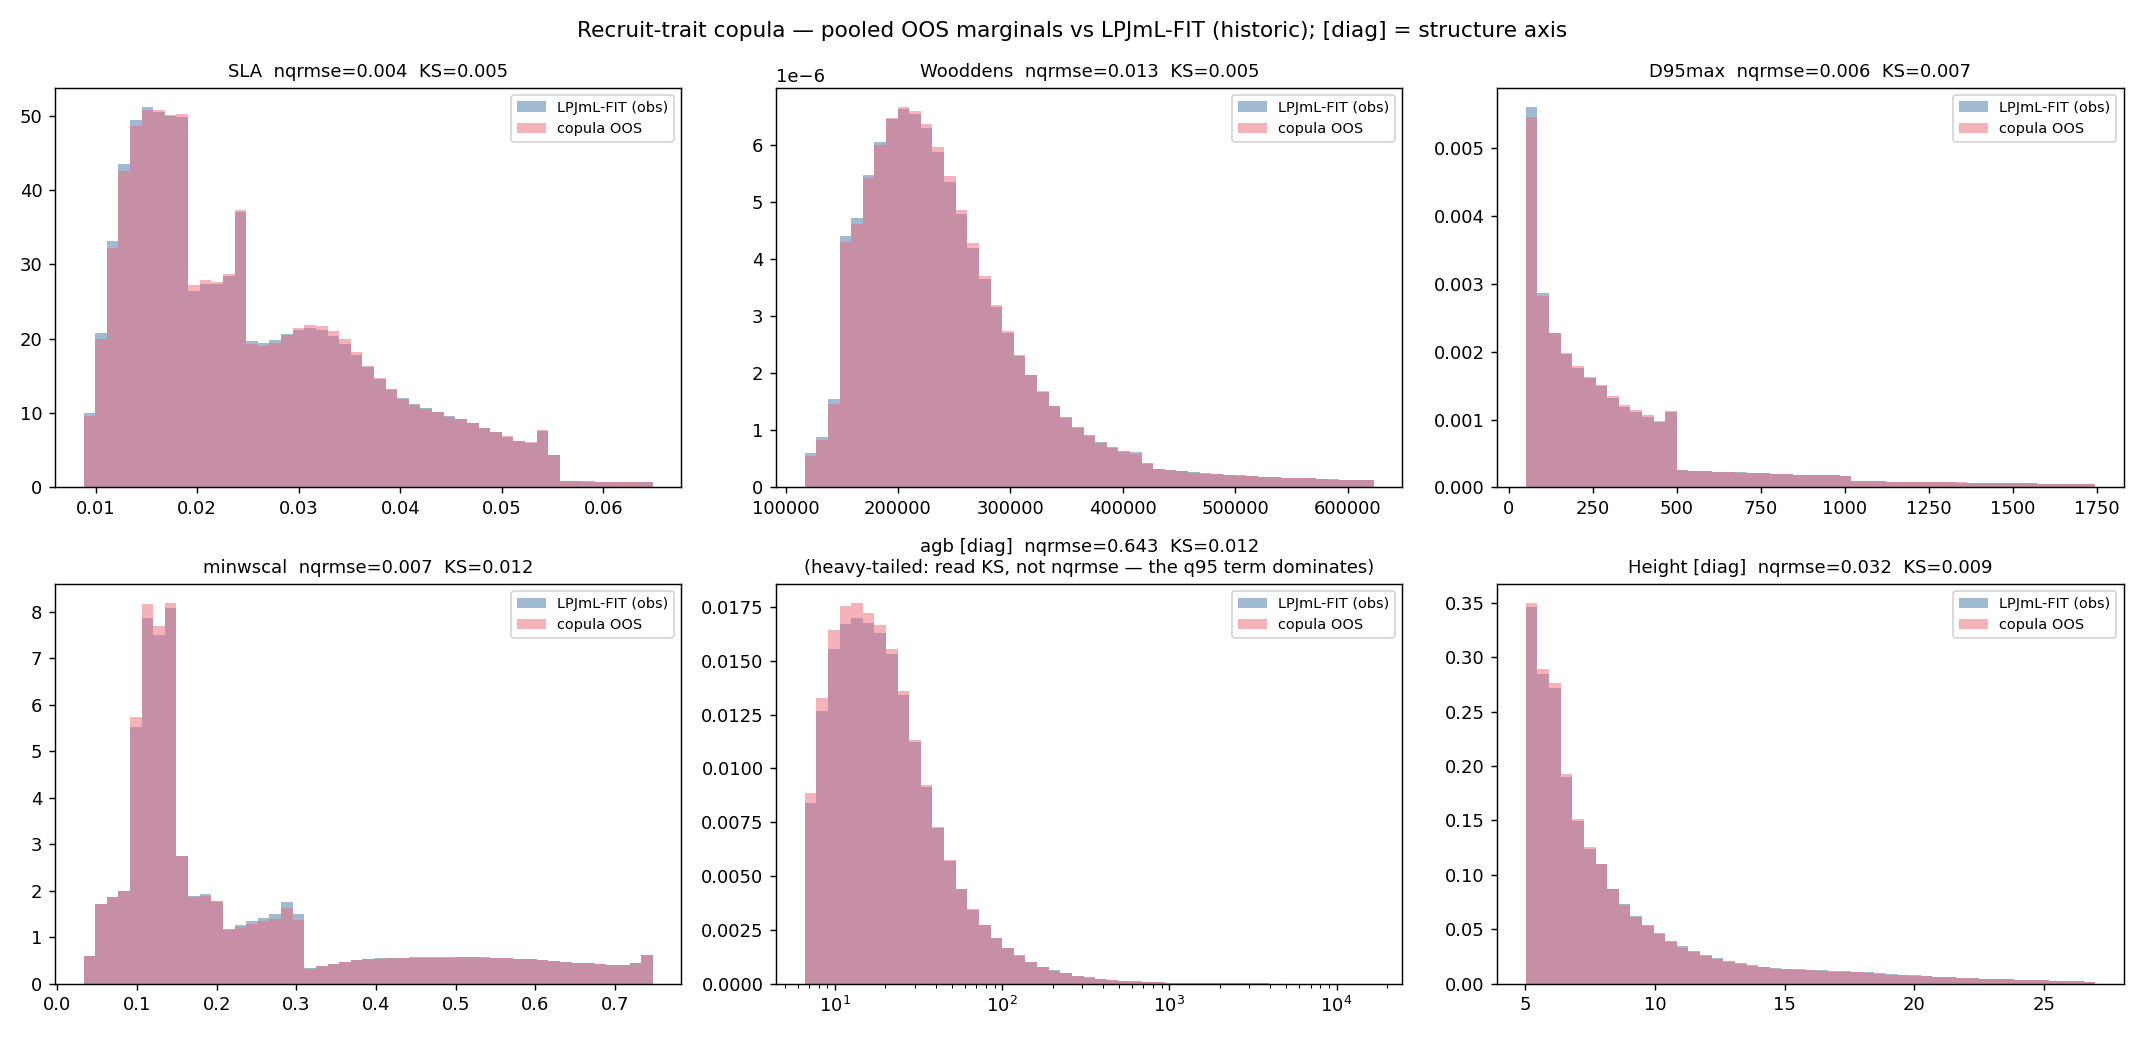
\includegraphics[width=\textwidth]{trait_marginals.png}
\caption[Global trait distributions, true versus predicted]{\textbf{What is shown.} Six panels, one per axis, each comparing the global distribution of that quantity -- how often each value occurs across all withheld trees -- for LPJmL-FIT versus Component S. Horizontal axis is the value in its own units; vertical axis is frequency.

\textbf{The axes.} Four \emph{live} axes are assigned by the running model: \textbf{SLA} (specific leaf area, leaf area per unit leaf mass -- thin light-catching versus thick durable leaves); \textbf{Wooddens} (wood density, trading fast growth against strength and longevity); \textbf{D95max} (rooting depth, above which 95\,\% of roots sit); \textbf{minwscal} (drought tolerance, the driest soil condition the tree still functions at, lower = more tolerant). Two panels marked \textbf{[diag]} are diagnostic: \textbf{agb} (above-ground biomass) and \textbf{Height}. Diagnostic axes are validated but not written into the production artifact, so errors in them cannot enter a coupled run.

\textbf{The printed numbers.} \textbf{nqrmse} is typical error as a fraction of the quantity's own interquartile range (smaller is better, comparable across units). \textbf{KS} is the largest gap between the two cumulative curves (0 = identical).

\textbf{What it tells us.} Both statistics are small and the curves overlap in all six panels, so the global shape of every trait is correct -- not merely the mean. The \texttt{agb} panel's nqrmse of $\approx 0.64$ is an artifact of the measure, not the model: biomass is strongly heavy-tailed and normalising by interquartile range is inappropriate for it; that panel's KS of $\approx 0.01$ is the meaningful figure. Being a pooled comparison, this figure cannot detect traits placed in the wrong \emph{regions}; the next two figures address that.}
\label{fig:trait_marginals}
\end{figure}

\begin{figure}[ht]
\centering
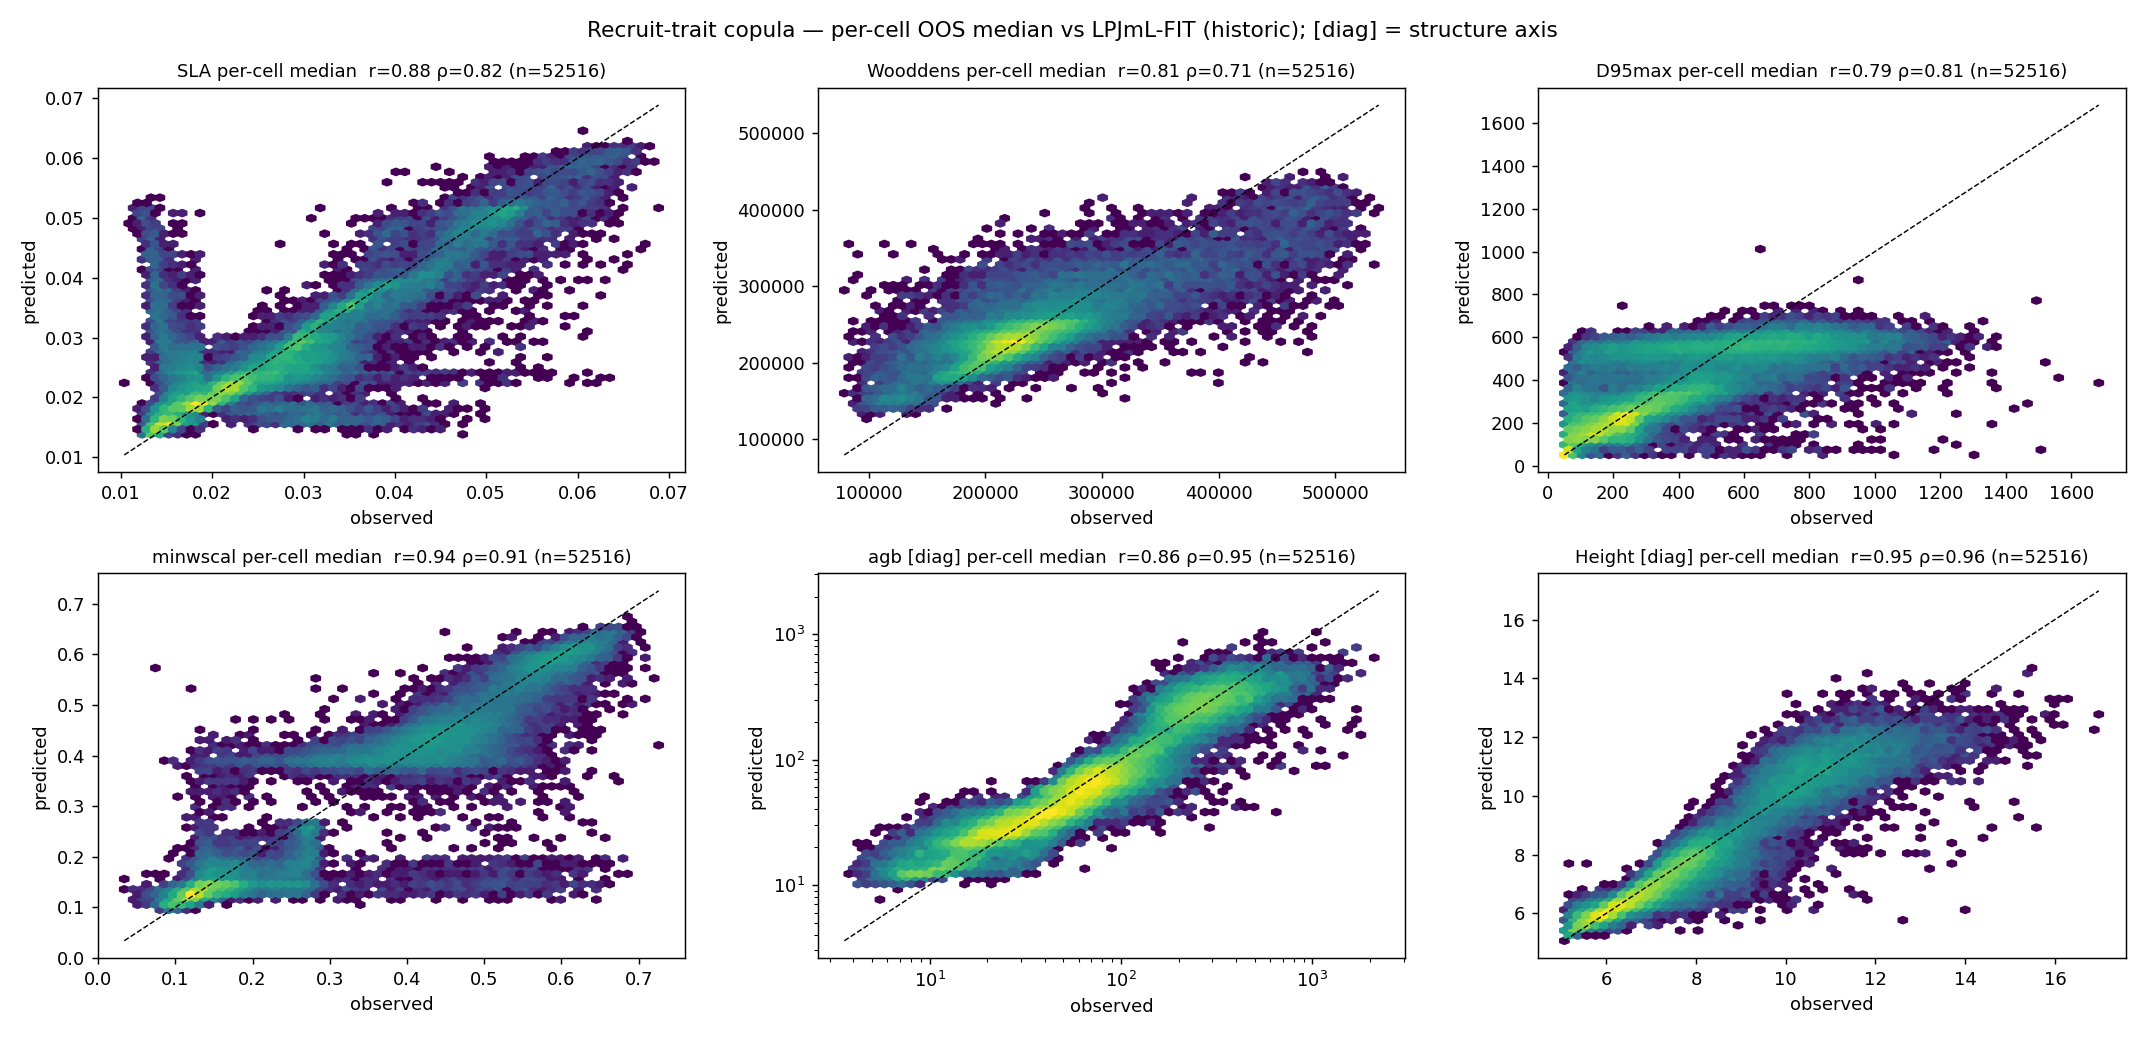
\includegraphics[width=\textwidth]{trait_percell_median.png}
\caption[Per-cell predicted versus true trait medians]{\textbf{What is shown.} The same six axes resolved to individual locations. Each dot is one of 52{,}516 grid cells: horizontal position is the true \emph{median} trait value among that cell's trees, vertical position the held-out predicted median, dashed line perfect agreement. The median (middle value when all trees at a cell are ranked) is used rather than the mean because it is not distorted by a few extreme individuals. Axis abbreviations as in Figure \ref{fig:trait_marginals}.

\textbf{What it tells us.} This tests whether the right traits are in the right \emph{places}, which Figure \ref{fig:trait_marginals} cannot. Drought tolerance, biomass and height track the diagonal closely. \textbf{Wood density is visibly the noisiest live axis}, with a wider cloud and mild flattening at both ends -- genuinely dense-wood locations are somewhat under-predicted and light-wood locations over-predicted. That flattening \emph{is} the low prediction-spread ratio of 0.678 in Table \ref{tab:traits}: the model hedges toward the middle rather than committing to extremes. Rooting depth shows a weaker version of the same behaviour.}
\label{fig:trait_percell}
\end{figure}

\begin{figure}[ht]
\centering
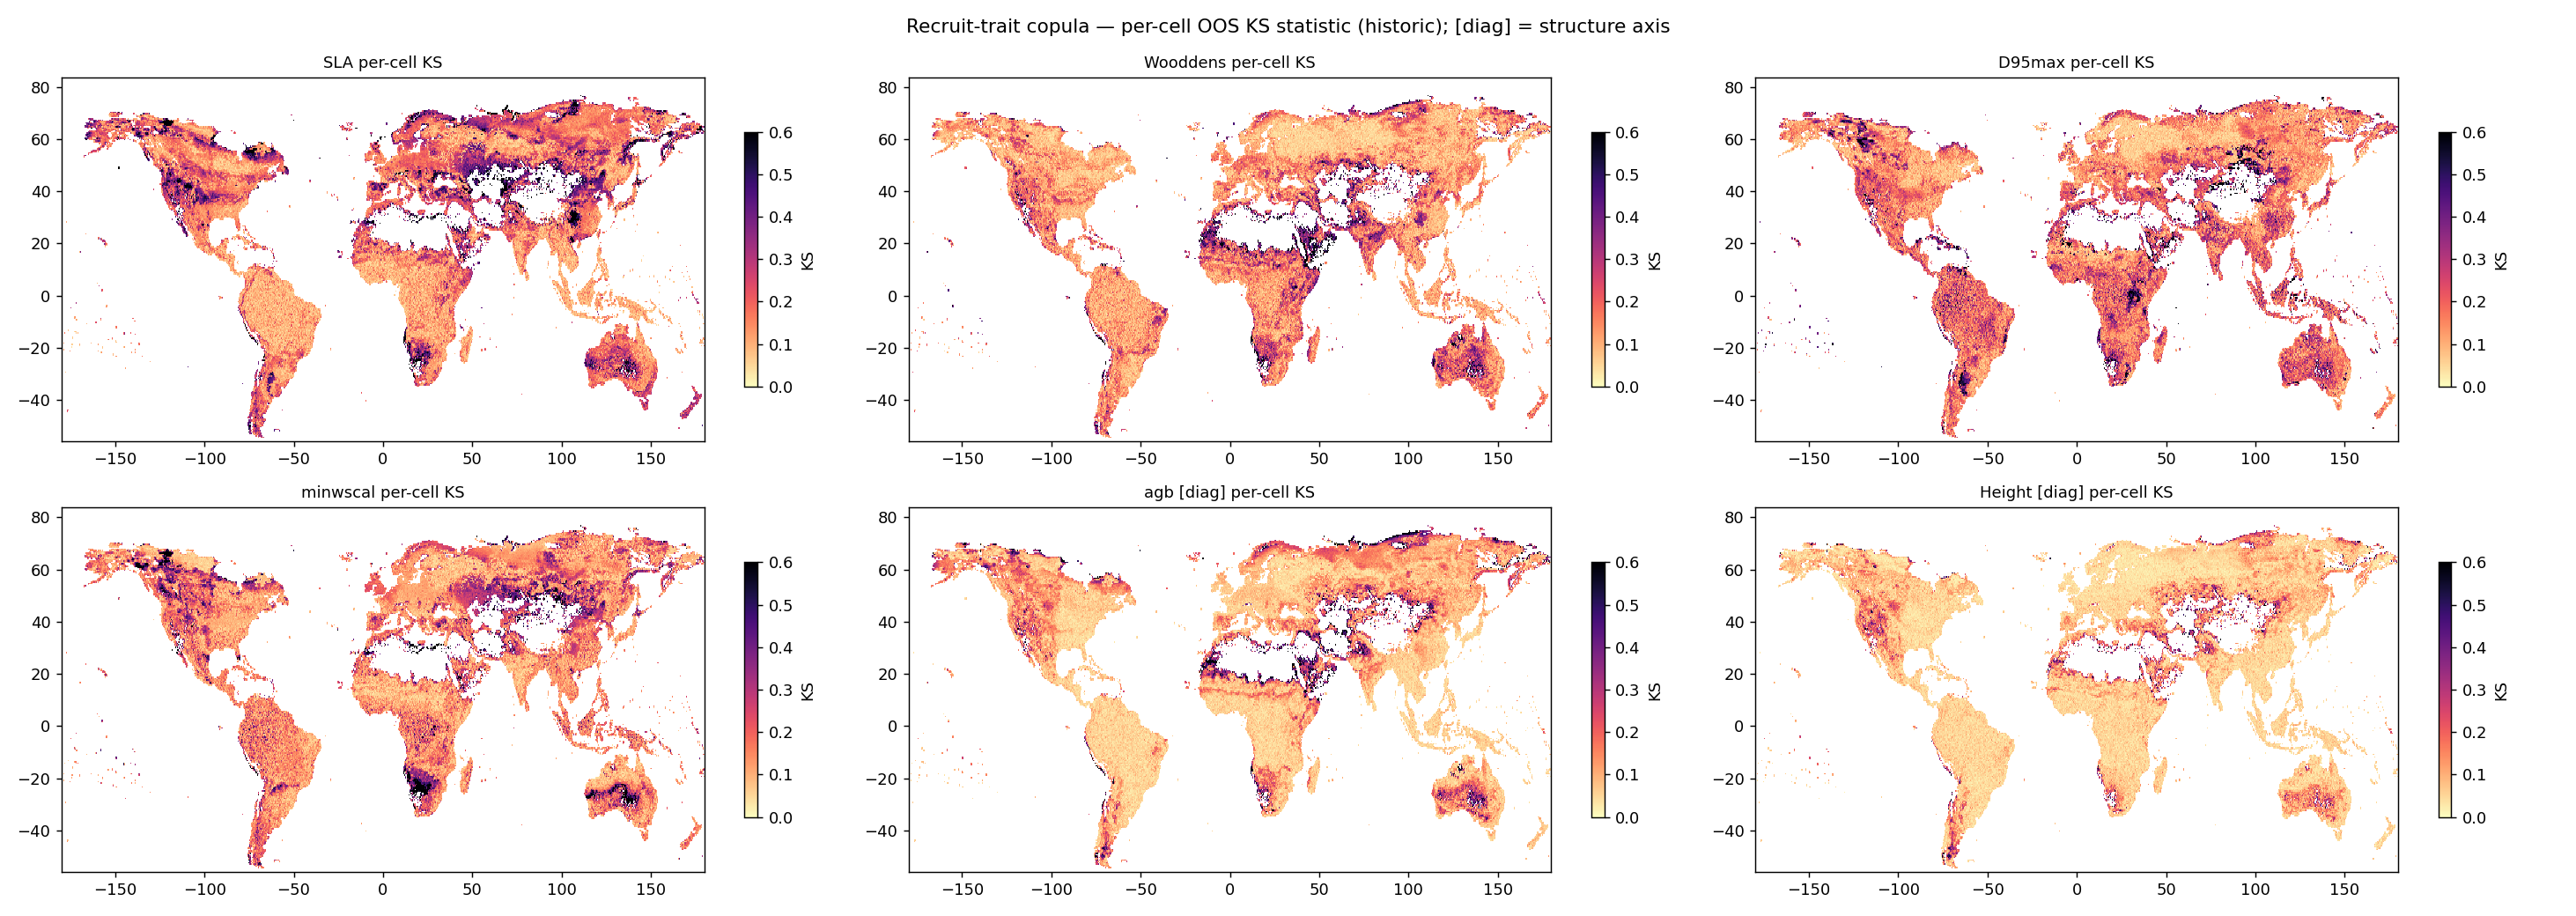
\includegraphics[width=\textwidth]{trait_ks_map.png}
\caption[Per-cell trait goodness-of-fit, mapped]{\textbf{What is shown.} Local goodness-of-fit mapped geographically, one panel per axis. Each cell's colour is its own Kolmogorov--Smirnov distance -- the largest discrepancy between predicted and true trait distributions \emph{at that cell alone} (0 = perfect local match). Pale = good, dark = poorer.

\textbf{Why this in addition to Figure \ref{fig:trait_percell}.} That figure compares only each cell's single middle value. This compares the \emph{entire local distribution}, so it detects cells where the median is right but the mix of trees around it is wrong -- and shows where on Earth that happens.

\textbf{What it tells us.} Most land is pale on all six axes: local trait distributions are reproduced well nearly everywhere. The informative feature is that poorer regions \emph{recur in the same places across several axes at once} rather than appearing independently -- evidence of a common cause, most plausibly that the current environmental predictors do not fully capture what sets local forest composition there, rather than unrelated noise. This identifies where additional predictors would most plausibly help. Per-cell KS values ($\approx 0.13$--$0.17$) are necessarily larger than the pooled values of Figure \ref{fig:trait_marginals} ($\approx 0.005$) because one cell holds far fewer trees; the two scales are not comparable.}
\label{fig:trait_ks_map}
\end{figure}

\clearpage
\subsection{Stand biomass and size: an end-to-end consistency check}

Stand biomass depends jointly on \emph{both} sub-models -- how many trees, and how large each is -- so it tests their mutual consistency in a way neither sub-model's own metrics can. It is diagnostic: it is not consumed by the coupled model.

\begin{table}[h]
\centering
\caption{Stand above-ground biomass, historical period, 53{,}699 cells.}
\label{tab:biomass}
\small
\begin{tabular}{lc}
\toprule
Metric & Value \\
\midrule
Per-cell $R^2$ & 0.931 \\
Per-cell $R^2$ (log$_{10}$ scale) & 0.945 \\
Median ratio, predicted / true & 1.020 \\
Global mean, observed vs predicted (gC\,m$^{-2}$) & 4452 vs 4178 \\
\bottomrule
\end{tabular}
\end{table}

\begin{figure}[ht]
\centering
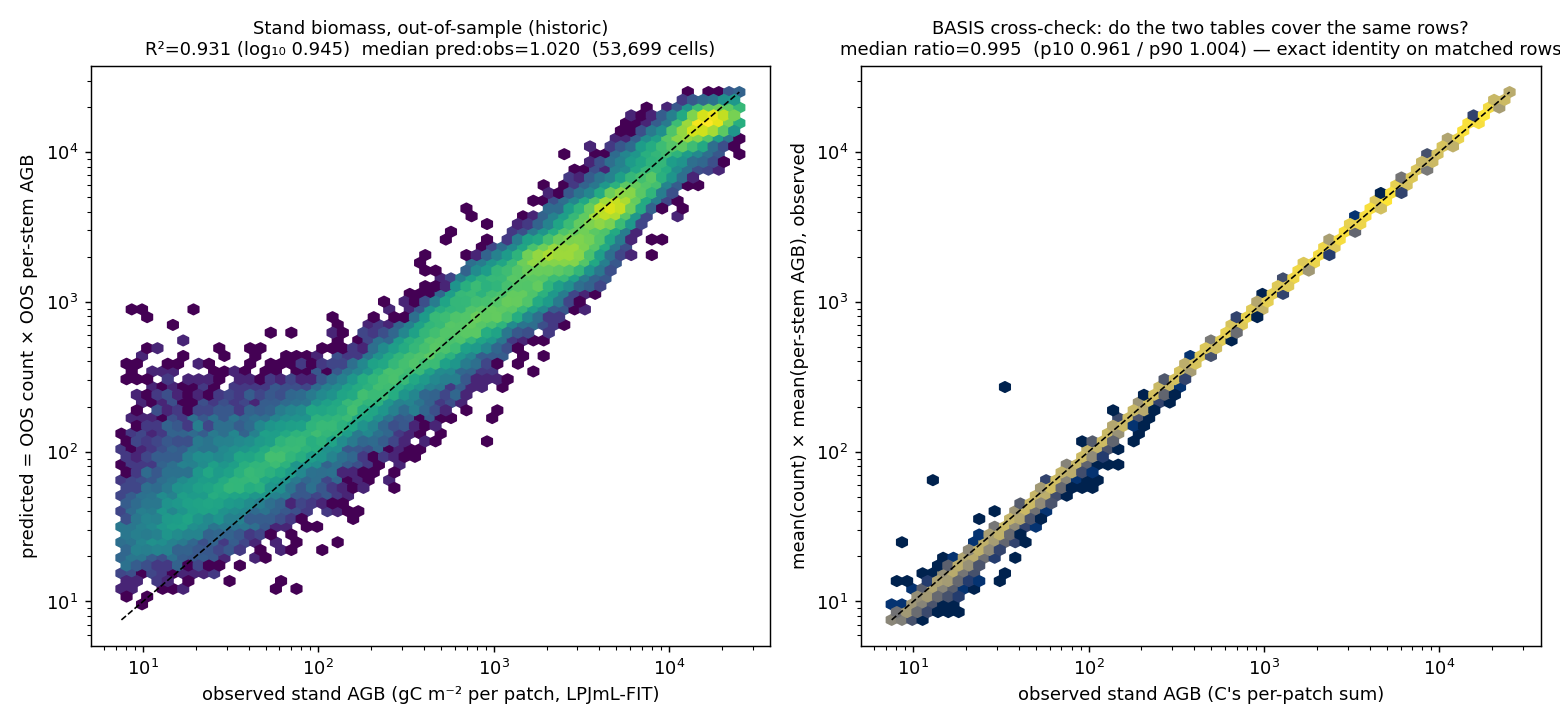
\includegraphics[width=0.95\textwidth]{biomass_percell.png}
\caption[Per-cell predicted versus true stand biomass]{\textbf{What is shown.} Predicted versus true stand above-ground biomass, one dot per grid cell, dashed diagonal for perfect agreement. ``Stand-level'' means summed over all trees in the patch, as opposed to the per-tree distributions of Figures \ref{fig:trait_marginals}--\ref{fig:trait_ks_map}. Above-ground biomass excludes roots.

\textbf{What it tells us.} The relationship is tight ($R^2 = 0.931$, rising to $0.945$ on a logarithmic scale, which reduces the leverage of a few extremely high-biomass tropical cells). The \emph{typical} cell is over-predicted by 2\,\% (median ratio 1.020) while the \emph{global mean} is under-predicted by about 6\,\%. These are consistent, and the difference between them is informative: it is the signature of a heavy-tailed quantity in which the few very-high-biomass cells are under-predicted while most ordinary cells are marginally over-predicted -- the same mild hedging toward the middle seen for wood density in Figure \ref{fig:trait_percell}. The two sub-models are therefore mutually consistent rather than compensating for each other's errors.}
\label{fig:biomass_percell}
\end{figure}

\begin{figure}[ht]
\centering
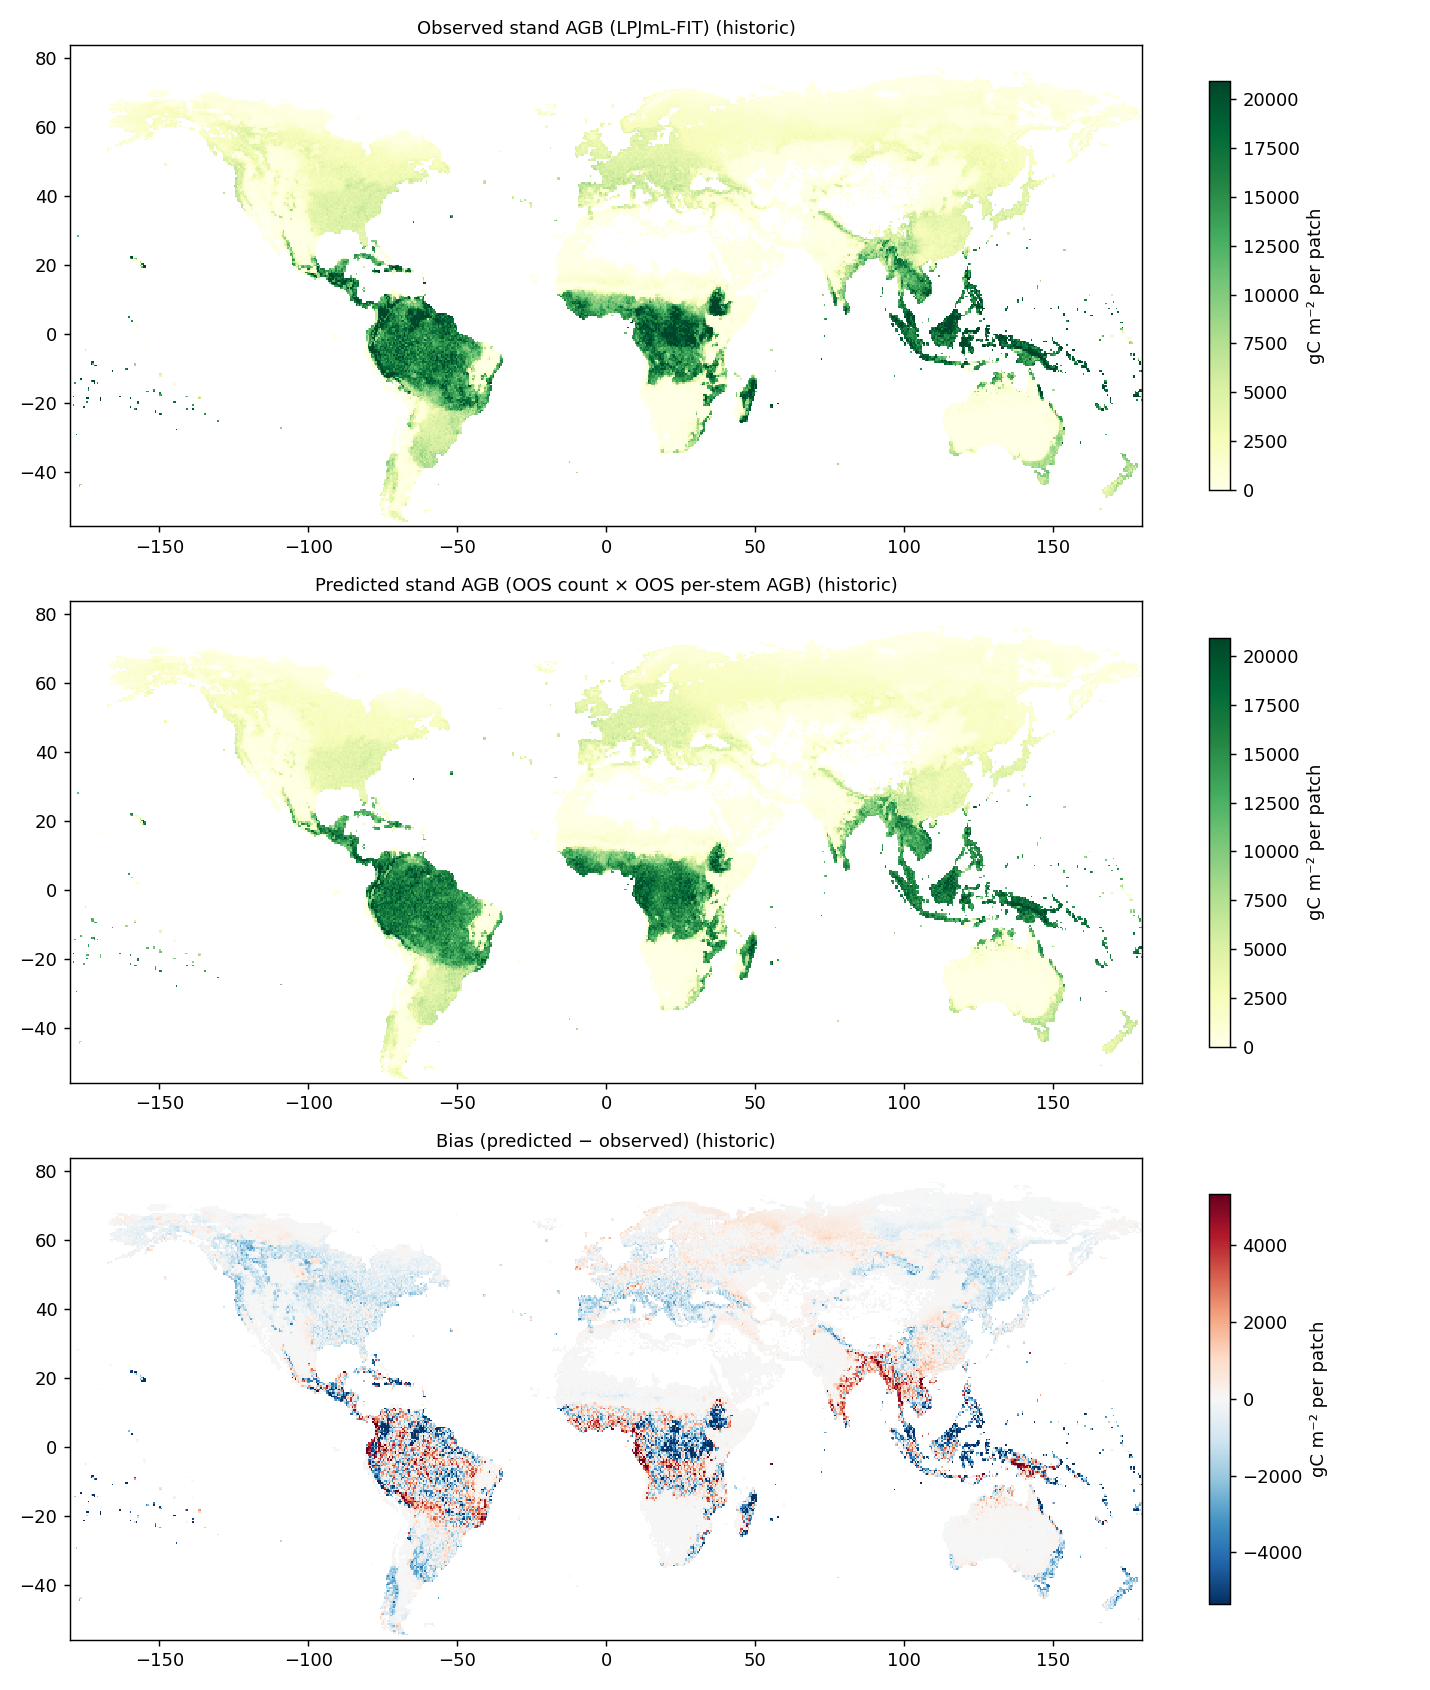
\includegraphics[width=0.85\textwidth]{biomass_maps.png}
\caption[Stand biomass, observed versus predicted, mapped]{\textbf{What is shown.} The stand biomass of Figure \ref{fig:biomass_percell} laid out geographically, observed and predicted side by side on a shared colour scale, with longitude and latitude as axes. Brighter = more biomass per unit area.

\textbf{What it tells us.} The large-scale pattern is reproduced: high-biomass tropical rainforest, intermediate temperate and boreal forest, near-zero arid and ice-covered regions. This is the spatial complement to Figure \ref{fig:biomass_percell} -- the scatter establishes numerical consistency between the two sub-models, and this figure establishes that the consistency is not achieved by regional errors cancelling in the global statistics, which a pooled scatter alone cannot exclude. Since biomass combines predicted tree number with predicted tree size, agreement at this scale is a meaningful end-to-end check -- of structural state, not of response to warming.}
\label{fig:biomass_maps}
\end{figure}

\clearpage
\section{Where Component S stands}
\label{sec:standing}

\subsection{Established capability}

\begin{itemize}[leftmargin=1.4em]
\item \textbf{Global forest structure, at or near the attainable ceiling.} Tree density at $R^2 = 0.982$ per patch-year and $0.999$ per cell; all four trait distributions matching in global shape (pooled KS $\le 0.012$) and at most individual locations; stand biomass consistent end-to-end at $R^2 = 0.931$.
\item \textbf{Transfer to an unseen climate regime.} Held-out-by-period accuracy matches held-out-by-location accuracy for counts, and trait fidelity is equal or better under SSP3-7.0 than historically.
\item \textbf{Complete PFT coverage} -- all seven tree types, 58{,}588 cells, both scenarios.
\item \textbf{A verified stochastic reference.} Two genuinely independent seeds exist for both scenarios, so the noise floor and hence the attainable ceiling are measured rather than assumed.
\item \textbf{Deployable artifacts.} Dependency-free serialised models (52\,MB counts, 129\,MB traits) that load in seconds and carry their own input-order contract, so a mismatch with the calling model is rejected at construction rather than producing silently wrong recruits.
\end{itemize}

\subsection{The skill is environmental response, not spatial lookup}

Because the standard hold-out scatters withheld cells among trained neighbours, part of the apparent skill could in principle be spatial interpolation. Testing this directly with contiguous blocked hold-out (design 2 of Section \ref{sec:validation}):

\begin{itemize}[leftmargin=1.4em]
\item A deliberately constructed \emph{position-only} model -- given latitude and longitude and nothing else -- scores $r = 0.837$ for wood density under scattered hold-out but collapses to $0.14$--$0.21$ under blocked hold-out. A model that knows only ``where am I'' cannot understand forests, yet under the scattered design it appeared competitive. This calibrates how much of a scattered-fold score can be interpolation.
\item The real environmental predictors retain about \textbf{73\,\%} of their scattered-fold skill under blocking ($0.811 \rightarrow 0.594$), against \textbf{21\,\%} for the position-only control. Most of what Component S knows is therefore transferable environmental response.
\end{itemize}

Consequently the headline numbers of Section \ref{sec:results} should be read as accuracy at a location whose neighbours are known -- which is the operationally relevant quantity, since the component runs on a fixed global grid where neighbours always exist -- and not as extrapolation into an unsurveyed region.

\subsection{The principal limitation: warming response is damped}
\label{sec:damping}

Reproducing a quantity's \emph{level} and reproducing its \emph{change} are different problems, and Component S is presently much better at the first.

The reason they differ is one of magnitude. The spatial contrast between a cold cell and a hot cell is large; the change at a single cell between the historical period and 2100 is small -- measured at only 20--31\,\% of the spatial signal. A correlation computed across all locations is therefore dominated by spatial contrast and is roughly three to five times less sensitive to the warming response. A high $R^2$ can coexist with a poorly reproduced response, and will barely register it.

Isolating the response gives:

\begin{itemize}[leftmargin=1.4em]
\item \textbf{The warming-driven shift in wood density is understated by $\approx 37$\,\%.} LPJmL-FIT shows a mean shift of $+2433$ (internal units); Component S predicts the same direction but about 892 units less, i.e.\ $\approx +1541$. The direction is right; the magnitude is not.
\item \textbf{The spatial pattern of the change is 24--62\,\% captured}, against a self-consistency ceiling of 0.87--0.96 -- so the pattern is genuinely present in the data and learnable, not noise.
\item The damping is a property of the current approach rather than of any optional extra input: the deployed 8-predictor configuration damps by 39.9\,\% on its own.
\end{itemize}

One methodological consequence is worth stating for anyone proposing a fix: reducing the damping is \emph{not} by itself evidence of improvement. A zero-information control model exhibits the least damping of any variant tested while having the worst response pattern. Any candidate must therefore be demonstrated on the response \emph{pattern} as well as its magnitude, under both hold-out designs.

\subsection{Reference-model repeatability declines for rooting depth under warming}

The noise floor is itself scenario-dependent, which bounds what any emulator can achieve:

\begin{table}[h]
\centering
\caption{Seed-to-seed reliability of LPJmL-FIT itself (how well one run predicts an independent rerun differing only in random seed), on a common basis of 57{,}295 cells. This is a property of the reference model, not of Component S.}
\label{tab:floor}
\small
\begin{tabular}{lccc}
\toprule
Trait & Historical & Future climate & $\Delta$ \\
\midrule
\texttt{SLA} & 0.965 & 0.975 & $+0.010$ \\
\texttt{Wooddens} & 0.923 & 0.944 & $+0.021$ \\
\textbf{\texttt{D95max}} & \textbf{0.895} & \textbf{0.837} & $\mathbf{-0.058}$ \\
\texttt{minwscal} & 0.973 & 0.978 & $+0.005$ \\
\bottomrule
\end{tabular}
\end{table}

The future period averages each cell over 81 years against 20 historically, so more averaging should raise reliability \emph{mechanically} on every axis. Three axes do. Rooting depth falls by 0.058 \emph{despite} that, meaning the true decline is larger than shown: under warming, two equally valid runs of the reference model disagree more about rooting depth than they do historically. Rooting-depth projections under warming therefore warrant more caution than the historical numbers alone imply -- a limit imposed by the reference model, independent of the emulator.

\subsection{Summary of status}

\begin{table}[h]
\centering
\caption{What is and is not established.}
\label{tab:status}
\small
\begin{tabular}{p{5.6cm}p{9.4cm}}
\toprule
\textbf{Established} & Global forest structure -- density, trait distributions, stand biomass -- at or near the attainable ceiling, one year at a time, at grid locations with known neighbours, on the complete tree PFT set and both scenarios. \\
\addlinespace
\textbf{Established with a stated correction} & The skill is transferable environmental response, not spatial lookup: $\approx 73$\,\% retained under blocked hold-out versus $21$\,\% for a position-only control. The margin is smaller than raw scores imply. \\
\addlinespace
\textbf{Not established} & Fidelity of the \emph{response to warming}: currently damped by $\approx 37$\,\%. \\
\addlinespace
\textbf{Not yet tested} & Recursive stability -- behaviour when called every year inside a live coupled simulation, with each year's output feeding the next. No result here addresses it. \\
\bottomrule
\end{tabular}
\end{table}

Component S is a validated \emph{structural} emulator and a not-yet-validated \emph{response} emulator. For applications requiring present-day or scenario-endpoint forest structure, the evidence supports use now. For applications whose conclusion depends on the magnitude of forest change under warming, Section \ref{sec:damping} is a live limitation that should govern interpretation.

\section{Remaining work, and how the objective is reached}
\label{sec:roadmap}

The objective is a land component that runs online inside an Earth System Model, reproducing LPJmL-FIT's forest dynamics faithfully at a small fraction of its cost. Four steps remain, in priority order.

\paragraph{1. Close the warming-response gap (Section \ref{sec:damping}).}
This is the scientific priority. A candidate exists and has been measured. Widening the trait model's predictors from 8 to 14 by adding the six moisture descriptors of Table \ref{tab:trait_inputs}, together with quantile-weighted forests and greater capacity, meets the project's formal trait criteria for the first time -- wood-density skill 0.901 and 58\,\% of the gap to the ceiling closed, with spread ratio rising to 0.854 and distributional fidelity improving on all four axes.

It has nevertheless \emph{not} been promoted to production, for a specific and instructive reason: those six descriptors are present-day climatological means, constant within each cell, so they cannot by construction encode a warming response -- a cell's historical and future rows are identical on them. Under blocked hold-out the wider set buys $+0.032$ of location-level skill while its apparent benefit for the response \emph{reverses sign}. It improves the quantity already near ceiling and does not improve the quantity that is not.

The intended resolution is therefore a \emph{scenario- and time-resolved} version of those moisture descriptors, recomputed per cell and per year from the underlying climate forcing rather than frozen at present-day means, so that the added information can carry a warming signal. This is specified but not yet built, and it is the single highest-value piece of remaining work.

\paragraph{2. Complete the ceiling measurement.}
A per-patch-year count noise floor, matched to what the count model actually predicts, is needed so that count accuracy can be stated relative to the attainable ceiling as trait accuracy already is. The trait ceiling under future climate additionally requires a seed-pair trait table built without the subsampling currently used for tractability, since the subsample is seed-dependent and would otherwise depress the floor and flatter the emulator.

\paragraph{3. Demonstrate recursive stability in the coupled model.}
Every number in this report is a single annual step evaluated against recorded outcomes, using the reference model's own drivers. The operational configuration instead feeds each year's emulated forest into the next year's physics. Establishing that errors do not accumulate across decades of such steps is a property of the coupled system and is the next milestone for the multi-cell coupled configuration, which consumes the artifacts described in Table \ref{tab:dims}.

\paragraph{4. Extend scope.}
Grass demography is currently handled by component F and could be brought under the same emulation approach. Per-PFT rather than pooled trait structure, and joint trait-correlation validation beyond the marginal and per-cell distributional checks reported here, are natural refinements once items 1--3 are settled.

\section{Conclusion}

Component S replaces an explicit individual-tree demography calculation with two trained statistical models -- a distributional random forest for tree number, and a conditional Gaussian copula for correlated recruit traits -- learned from LPJmL-FIT output and validated out-of-sample against it.

It reproduces global forest structure at or close to the limit set by the reference model's own stochasticity, across all seven tree functional types, under both historical and SSP3-7.0 climate, and it does so through genuine environmental response rather than spatial lookup. Its deployable artifacts are compact and dependency-free.

Its warming response is damped by about 37 percent, its recursive behaviour inside a live coupled run is untested, and it covers trees only. The route to closing the first of these is identified and specified; the second is the next coupled-model milestone. On present evidence Component S is ready to supply forest structure to a coupled land model, and not yet ready to be the basis of a quantitative claim about the magnitude of forest change under warming.

\newpage
\section*{Glossary}
\addcontentsline{toc}{section}{Glossary}

\begin{description}[leftmargin=!,labelwidth=3.4cm,style=nextline]
\item[Above-ground biomass (agb)] Mass of trunk, branches and leaves above the soil, excluding roots.
\item[Copula] A construction that separates the individual distribution of each variable from the dependence structure between them, allowing correlated draws with correct marginals.
\item[Distributional random forest] A random forest whose leaves retain the full set of training values reaching them, so predictions are distributions rather than single numbers.
\item[Emulator] A fast statistical model trained to reproduce the input--output behaviour of a slower process model.
\item[Foliar projective cover (fpc)] The fraction of ground shaded by foliage when viewed from above.
\item[Growing-degree days (GDD5)] Accumulated daily temperature above 5\,$^\circ$C over a year; a measure of thermal growing-season length.
\item[Held-out (out-of-sample)] Evaluated on data withheld from the model being scored during its training.
\item[Leaf area index (LAI)] Leaf area per unit ground area.
\item[Noise floor] The accuracy limit imposed by the reference model's own stochasticity: how well one run predicts an independent rerun differing only in random seed.
\item[Patch] A small fixed-area unit of forest simulated independently; 25 per grid cell here, representing the natural spread of forest states.
\item[Plant functional type (PFT)] A class of plants grouped by shared physiology and structure (e.g.\ boreal needleleaved evergreen) rather than by species.
\item[Specific leaf area (SLA)] Leaf area per unit leaf mass; high values indicate thin, light-capturing leaves.
\item[SSP3-7.0] A high-emissions future scenario used for the future-climate period.
\item[Wood density] Mass of wood per unit volume; trades rapid growth against mechanical strength and longevity.
\end{description}

\end{document}
